 %%%%%%%%%%%%%%%%%%%%%%
\section{Numerical Experiments}
\label{sec:NumExp}

For our numerical experiments, we calculated normalized geodesic lengths for a variety of regression and classification tasks.  In practice, this involved training a pair of randomly initialized models to the desired test loss value/accuracy/perplexity, and then attempting to connect that pair of models via the Dynamic String Sampling algorithm.  We also tabulated the average number of ``beads'', or the number intermediate models needed by the algorithm to connect two initial models.  For all of the below experiments, the reported losses and accuracies are on a restricted test set.  For more complete architecture and implementation details, see our GitHub page.

The results are broadly organized by increasing model complexity and task difficulty, from easiest to hardest.  Throughout, and remarkably, we were able to easily connect models for every dataset investigated except the one explicitly constructed counterexample in section SYMMDISCONNECTHERE.  Qualitatively, all of the models exhibit a transition from a highly convex regime at high loss to a highly non-convex regime at low loss, as demonstrated by the growth of the normalized length as well as the number of required ``beads'' in each model.


\subsection{Polynomial Regression}
\label{sec:PolyFuncs}
%%%%%%%%%%%%%%%%%%%%%%

 We studied a 1-4-4-1 fully connected multilayer perceptron style architecture with sigmoid nonlinearities and RMSProp/ADAM optimization.  For ease-of-analysis, we restricted the training and test data to be strictly contained in the interval $x\in[0,1]$ and $f(x)\in[0,1]$.  The number of required beads, and thus the runtime of the algorithm, grew approximately as a power-law, as demonstrated in Figs. ref{QUADRATICSfigs} and \ref{CUBICfigs}.
 
 The cubic regression task exhibits an interesting feature around $L_0=.15$ in Fig. \ref{CUBICfigs}, where the normalized length spikes, but the number of required beads remains low.  Up until this point, the cubic model is strongly convex, so this first spike seems to indicate the onset of non-convex behavior and a concomitant radical change in the geometry of the loss surface for lower loss.
 

\begin{figure}
\label{QUADRATICSfigs}
\centering
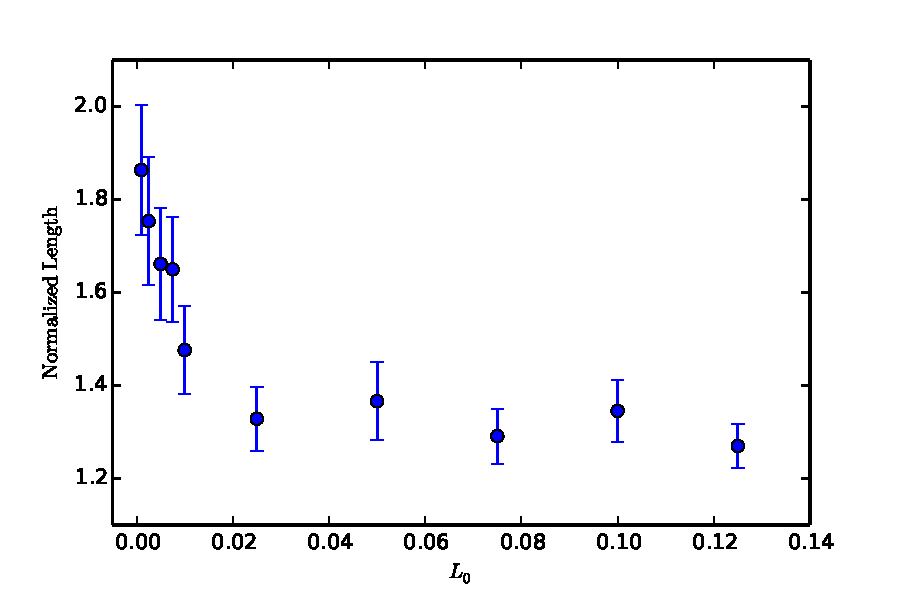
\includegraphics[width=.4\textwidth]{../Plots/normlengthquadratics}
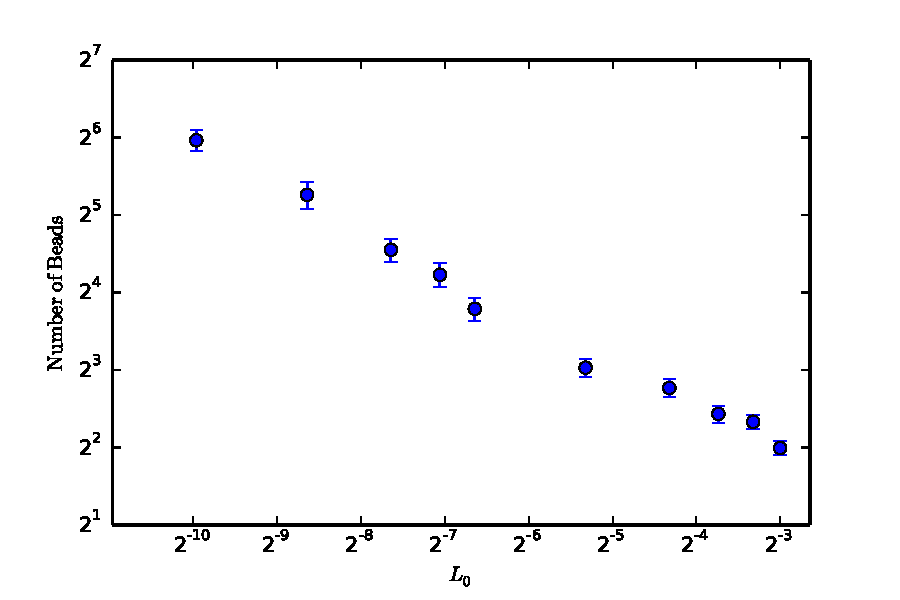
\includegraphics[width=.4\textwidth]{../Plots/numbeadsquadratics}
\caption{(Left) Average normalized geodesic length and (Right) average number of beads as a function of the energy level for a quadratic regression task.  The polynomial fitted was $f(x) = .5x^2 + .25x + .1$.}
\end{figure}
 
 
 \begin{figure}
\label{CUBICSfigs}
\centering
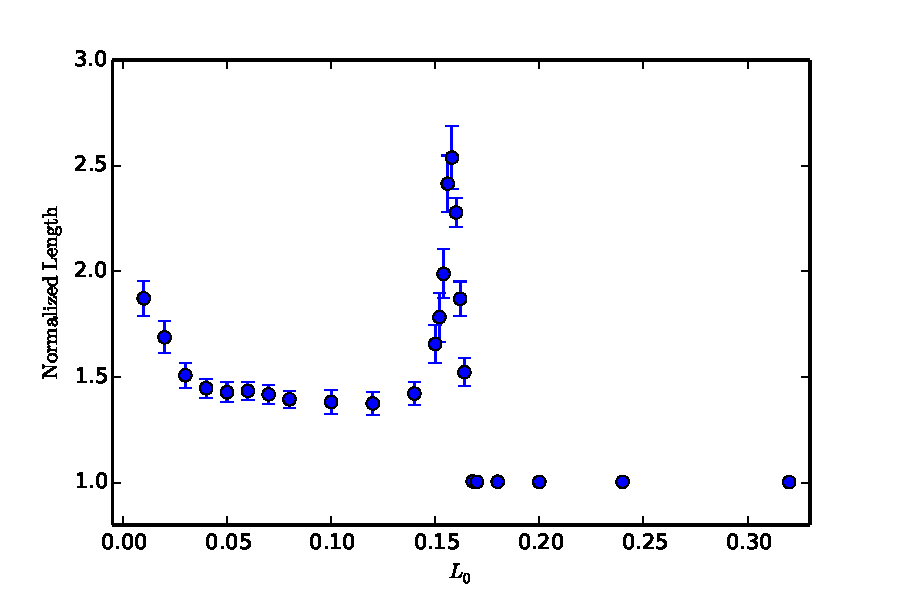
\includegraphics[width=.4\textwidth]{../Plots/normlengthcubics}
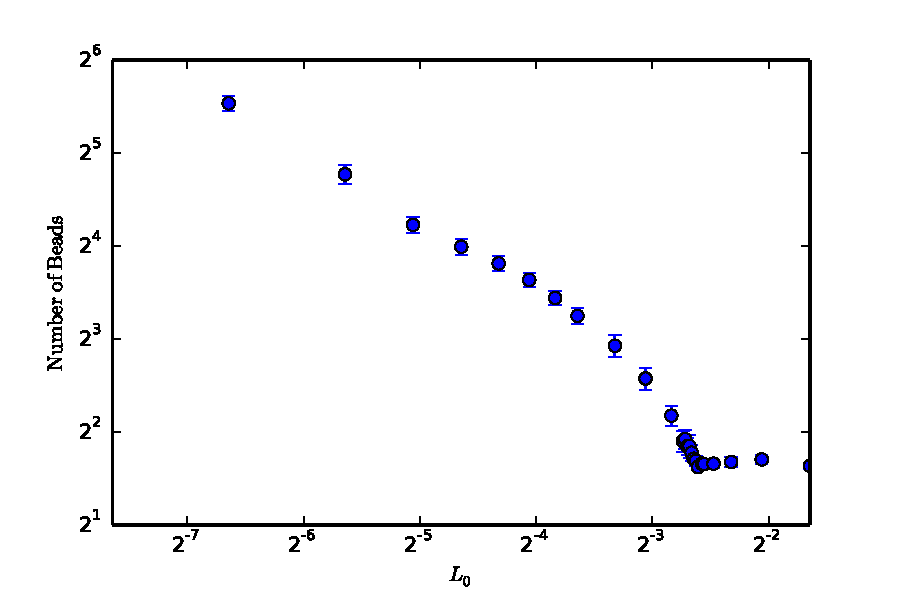
\includegraphics[width=.4\textwidth]{../Plots/numbeadscubics}
\caption{(Left) Average normalized geodesic length and (Right) average number of beads as a function of the energy level for a cubic regression task.  The polynomial fitted was $f(x) = 8x^3 -10x^2 + 3x$.}
\end{figure}

%%%%%%%%%%%%%%%%%%%%%%
\subsection{Convolutional Neural Networks}
\label{sec:CNN}
%%%%%%%%%%%%%%%%%%%%%%

 To test the algorithm on larger architectures, we ran it on the MNIST hand written digit recognition task as well as the CIFAR10 image recognition task.  Again, the data exhibits strong qualitative similarity with the previous models: normalized length remains low until a threshold loss value, after which it grows approximately as a power law.  Interestingly, the MNIST dataset exhibits very low normalized length, even for models nearly at the state of the art in classification power, in agreement with the folk-understanding that MNIST is highly convex and/or ``easy''.  The CIFAR10 dataset, however, exhibits large non-convexity, even at the modest test accuracy of 80%.

\begin{figure}
\label{MNISTfigs}
\centering
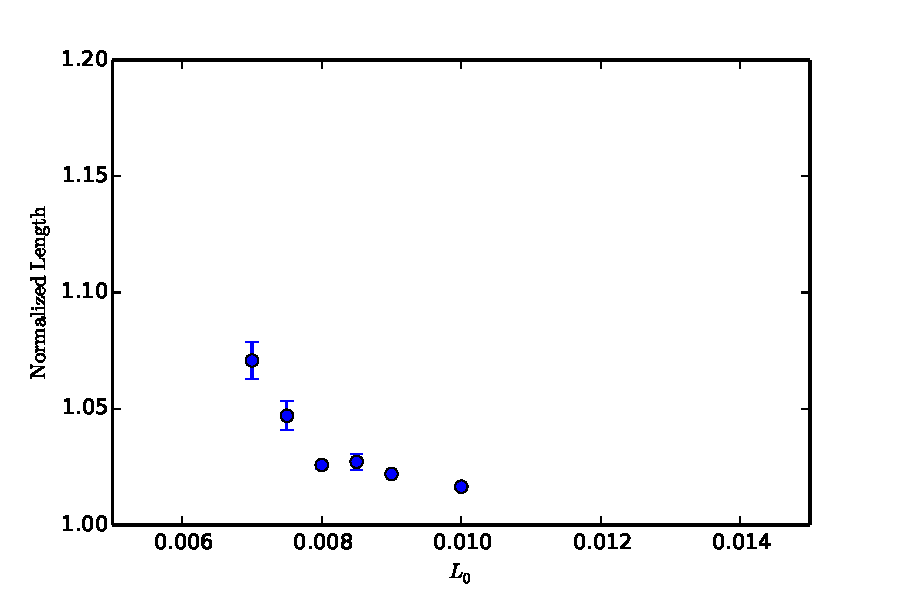
\includegraphics[width=.4\textwidth]{../Plots/normlengthMNIST}
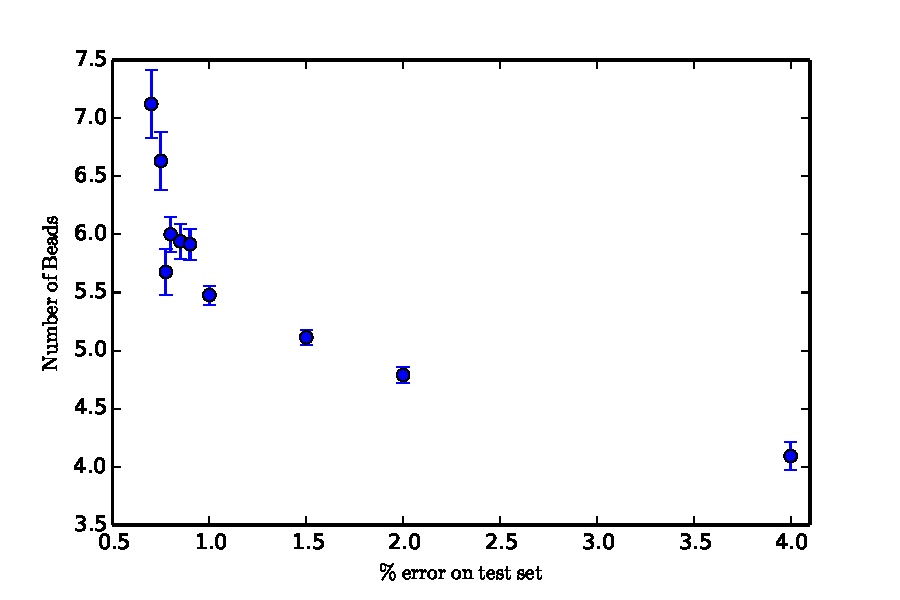
\includegraphics[width=.4\textwidth]{../Plots/numbeadsMNIST}
\caption{(Left) Average normalized geodesic length and (Right) average number of beads as a function of test accuracy for a CITESTYLE convnet architecture for MNIST hand digit recognition.}
\end{figure}


\begin{figure}
\label{CIFARfigs}
\centering
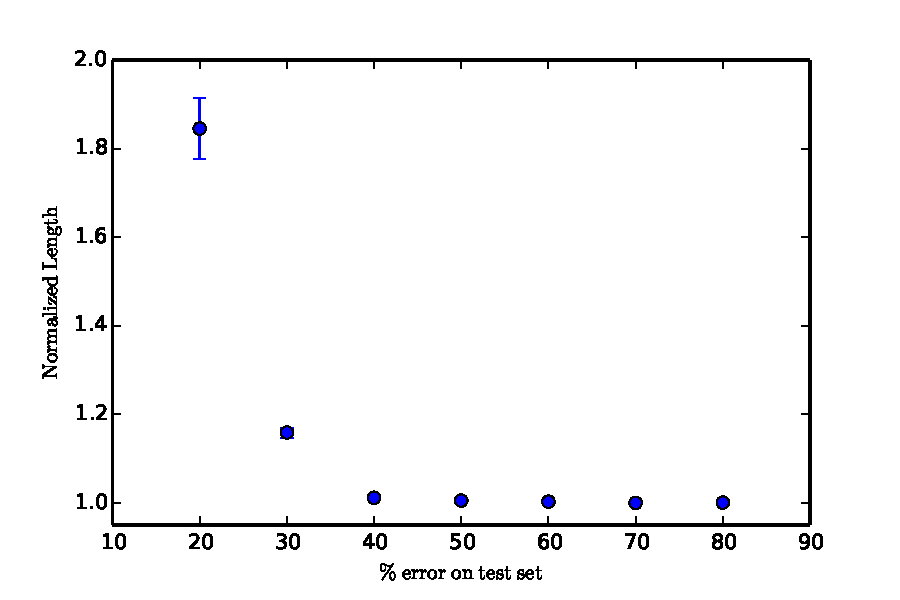
\includegraphics[width=.4\textwidth]{../Plots/normlengthCIFAR}
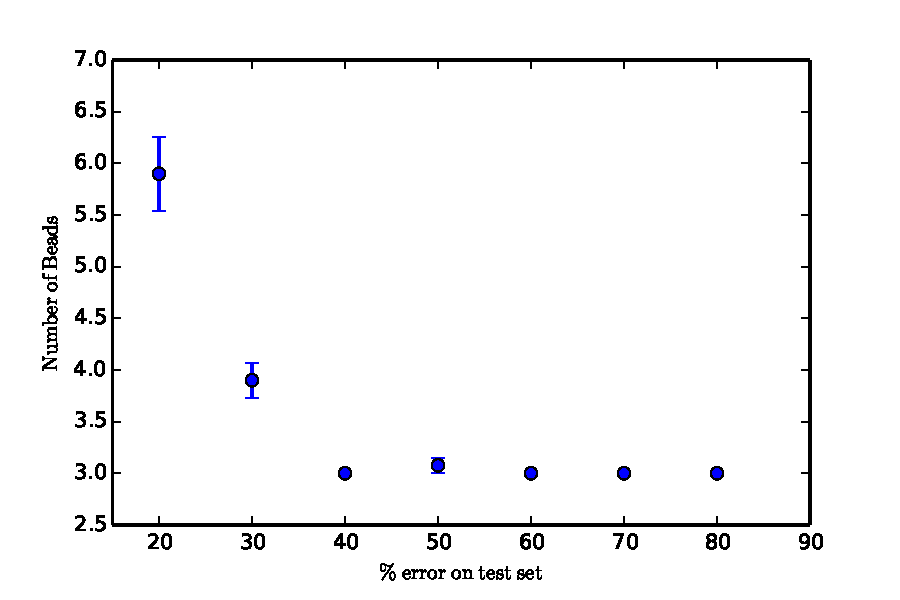
\includegraphics[width=.4\textwidth]{../Plots/numbeadsCIFAR}
\caption{(Left) Average normalized geodesic length and (Right) average number of beads as a function of the test accuracy for a CITESTYLE convnet architecture for CIFAR10 image classification.}
\end{figure}

%%%%%%%%%%%%%%%%%%%%%%
\subsection{Recurrent Neural Networks}
%%%%%%%%%%%%%%%%%%%%%%

 To gauge the generalizability of our algorithm, we also applied it to an LSTM architecture for solving the next word prediction task on the PTB dataset.

\begin{figure}
\label{PTBfigs}
\centering
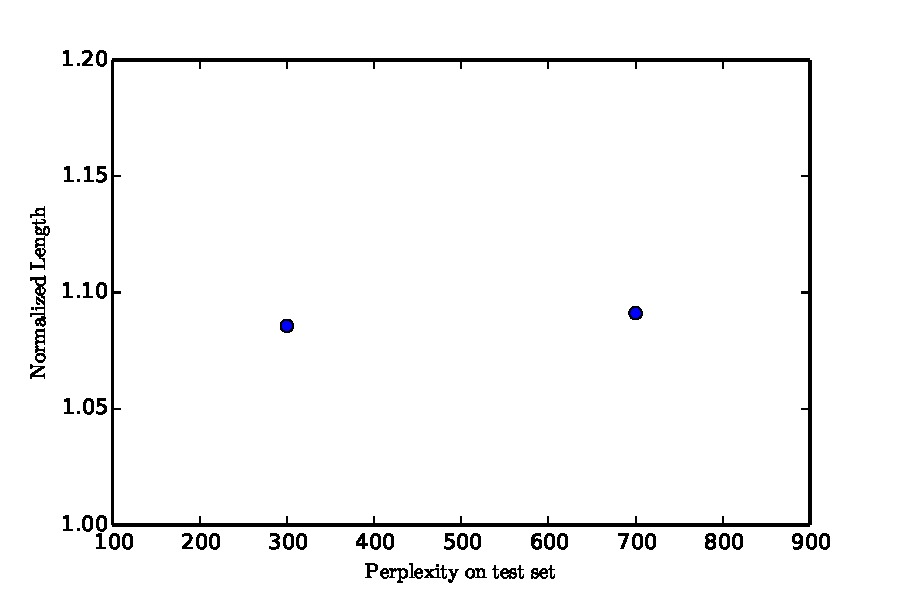
\includegraphics[width=.4\textwidth]{../Plots/normlengthPTB}
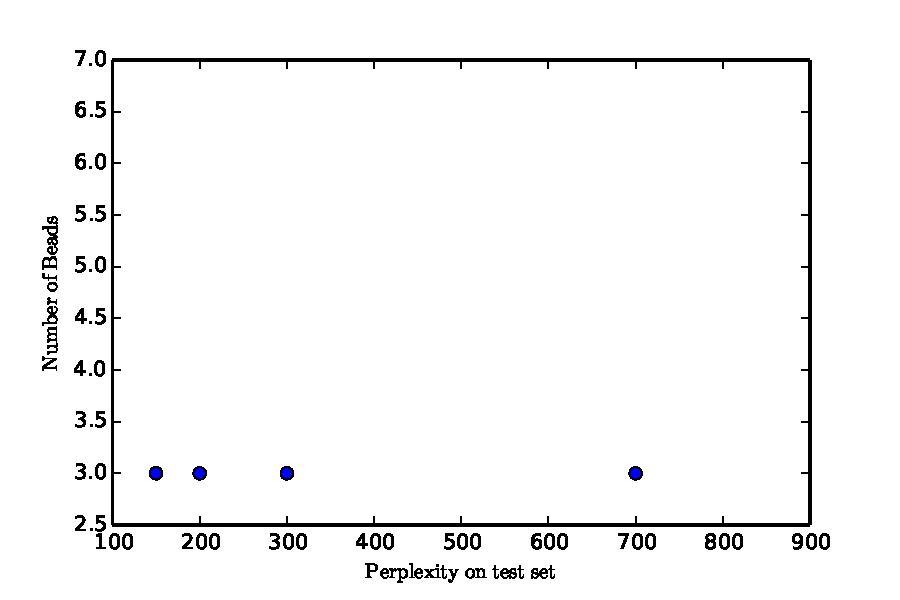
\includegraphics[width=.4\textwidth]{../Plots/numbeadsPTB}
\caption{(Left) Average normalized geodesic length and (Right) average number of beads as a function of perplexity for a 2-cell LSTM RNN for the PTB dataset for next word prediction.}
\end{figure}


